\documentclass[table]{beamer}

\usepackage{kotex}
\usepackage{amsmath}
\usepackage{amssymb}
\usepackage{verbatim}
\ifxetex
 \setsansfont{TeX Gyre Heros}
 \setsanshangulfont{맑은 고딕}
\fi
\usepackage{color, colortbl}					%tabular에서 rowcolor를 변경하기 위해서..
\usepackage{fancybox}
\usepackage{graphbox,graphicx}
\usepackage{tikz}								%오버레이에 그림을 그리기 위해서..
\usepackage{hyperref}							%하이퍼링크 처리

\usepackage{array}
\usepackage{ebproof}
\usepackage{multirow}


\usepackage{xcolor,multirow}
\usepackage{hhline}

\usepackage[T1]{fontenc}
\usepackage{textcomp}
\usepackage{listings}							%자바 코드를 위해서..
\lstset{
	mathescape,
	language=Java,
	basicstyle=\footnotesize\ttfamily,
	keywordstyle={}, % \footnotesize\color{blue}\ttfamily,
	captionpos=b,
	escapeinside=@@,
	showstringspaces=false,					%공백 문제 제거를 위해서
	tabsize=2,
	upquote=true
}

%----------------- 총 페이지수에서 백업 슬라이드를 제거하기 위해서....
\newcommand{\backupbegin}{
   \newcounter{framenumberappendix}
   \setcounter{framenumberappendix}{\value{framenumber}}
}
\newcommand{\backupend}{
   \addtocounter{framenumberappendix}{-\value{framenumber}}
   \addtocounter{framenumber}{\value{framenumberappendix}} 
}
%-----------------

%---------------- tabular에서 rowcolor를 변경하기 위해서..
\definecolor{Gray}{gray}{0.9}
%-----------------

%\usetheme{CambridgeUS}
% \usecolortheme{default}

\usetheme{default}
\usecolortheme{default}

%\usetheme{default}
%\usecolortheme{beaver}
%\usetheme{CambridgeUS}
%\usecolortheme{seagull}

%\useinnertheme{rectangles}


\setbeamertemplate{caption}{\insertcaption}	%그림의 캡션 자동 만들지 않도록.

\addtobeamertemplate{navigation symbols}{}{%
    \usebeamerfont{footline}%
    \usebeamercolor[fg]{footline}%
    \hspace{1em}%
    \insertframenumber/\inserttotalframenumber
}

\title[Types and Programming Languages]{3. Untyped Arithmetic Expressions \\
(Types and Programming Languages)}
\author[K. Choi]{Kwanghoon Choi}
\institute[Chonnam National University]{
Software Languages and Systems Laboratory \\
	Chonnam National University}
\date{Week 3}

%%%%% Macros %%%%%

\newcommand{\rpc}{$\lambda_{rpc}$}
\newcommand{\polyrpc}{$\lambda_{rpc}^{\forall}$}
\newcommand{\stateencrpc}{$\lambda_{rpc}^{enc}$}
\newcommand{\statefulrpc}{$\lambda_{rpc}^{state}$}

\newcommand{\cs}{$\lambda_{cs}$}
\newcommand{\stateenccs}{$\lambda_{cs}^{enc}$}
\newcommand{\statefulcs}{$\lambda_{cs}^{state}$}

\newcommand{\client}{\textbf{c}}
\newcommand{\server}{\textbf{s}}
\newcommand{\clientserver}{\textbf{cs}}

\newcommand{\Loc}{Loc}

\newcommand{\evalRPC}[3]{#1\Downarrow_{#2}#3}
\newcommand{\evalRPCC}[2]{#1\Downarrow_{\client}#2}
\newcommand{\evalRPCS}[2]{#1\Downarrow_{\server}#2}
\newcommand{\lamL}[3]{\lambda^{#1}#2.#3}
\newcommand{\appL}[3]{#1{\ }^{#2}#3} 
\newcommand{\subst}[2]{\{#1/#2\}}
\newcommand{\llet}[3]{\textsf{let} \ #1 = #2 \ \textsf{in} \ #3}

\newcommand{\textsfReq}{\textsf{req}}
\newcommand{\req}[2]{\textsfReq(#1,#2)}
\newcommand{\reqwith}[3]{\textsfReq_{#1}(#2,#3)}

\newcommand{\textsfCall}{\textsf{call}}
\newcommand{\call}[2]{\textsfCall(#1,#2)}
\newcommand{\callwith}[3]{\textsfCall_{#1}(#2,#3)}

\newcommand{\textsfRet}{\textsf{ret}}
\newcommand{\ret}[1]{\textsfRet(#1)}
\newcommand{\retwith}[2]{\textsfRet_{#1}(#2)}

\newcommand{\funL}[1]{\xrightarrow{#1}}    
\newcommand{\funLC}[2]{\xrightarrow[#2]{#1}}  
\newcommand{\tyenv}{\Gamma}     
\newcommand{\tyenvExt}[2]{\Gamma\{#1:#2\}}
\newcommand{\tyenvExtWith}[1]{\Gamma,#1}
% \newcommand{\typing}[4]{#1\rhd_{#2} #3 : #4}       
\newcommand{\typing}[4]{#1\vdash_{#2} #3 : #4}       
\newcommand{\typingBlack}[4]{#1\blacktriangleright_{#2} #3 : #4}  

\newcommand{\loceta}[2]{{#1}\rightsquigarrow{#2}}                                         

\newcommand{\enc}{\textsf{enc}}
\newcommand{\evalStateEncRPCC}[2]{$#1\Downarrow_{\client}^{\enc}#2$}
\newcommand{\evalStateEncRPCS}[3]{$#1;#2\Downarrow_{\server}^{\enc}#3$}

\newcommand{\sta}{\textsf{state}}
\newcommand{\evalStatefulRPCC}[3]{\evalStatefulRPC{#1}{#2}{\client}{#3}}
\newcommand{\evalStatefulRPCS}[3]{\evalStatefulRPC{#1}{#2}{\server}{#3}}
\newcommand{\evalStatefulRPC}[4]{${#1};{#2}\Downarrow_{#3}^{\sta}{#4}$}

\newcommand{\deep}{\textsf{deep}}
\newcommand{\evalDeeplyStatefulRPCC}[3]{\evalDeeplyStatefulRPC{#1}{#2}{\client}{#3}}
\newcommand{\evalDeeplyStatefulRPCS}[3]{\evalDeeplyStatefulRPC{#1}{#2}{\server}{#3}}
\newcommand{\evalDeeplyStatefulRPC}[4]{${#1};{#2}\Downarrow_{#3}^{\deep}{#4}$}

\newcommand{\IdK}{\textsf{Id}}
\newcommand{\FunK}[3]{\textsf{Fun} \ #2 \ #3}
\newcommand{\AppK}[3]{\textsf{App} \ #2 \ #3}
%\newcommand{\FunK}[3]{\textsf{Fun}^{#1} \ #2 \ #3}
%\newcommand{\AppK}[3]{\textsf{App}^{#1} \ #2 \ #3}
                                                
\newcommand{\reify}[1]{\ulcorner #1 \urcorner}

\newcommand{\RightarrowEnc}{\Rightarrow^{enc}}
\newcommand{\RightarrowEncStar}{\Rightarrow^{enc*}}
\newcommand{\RightarrowEncPlus}{\Rightarrow^{enc+}}

\newcommand{\runStateEncRPC}[2]{$#1 \RightarrowEnc #2$}
\newcommand{\runStateEncRPCStar}[2]{$#1 \RightarrowEncStar #2$}
\newcommand{\runStateEncRPCPlus}[2]{$#1 \RightarrowEncPlus #2$}

\newcommand{\runStateEncCS}[2]{$#1 \Rightarrow^{enc} #2$}
\newcommand{\runStateEncCSStar}[2]{$#1 \Rightarrow^{enc*} #2$}

\newcommand{\runStatefulRPC}[2]{$#1 \Rightarrow^{state} #2$}
\newcommand{\runStatefulRPCStar}[2]{$#1 \Rightarrow^{state*} #2$}

\newcommand{\runStatefulCS}[2]{$#1 \Rightarrow^{state} #2$}
\newcommand{\runStatefulCSStar}[2]{$#1 \Rightarrow^{state*} #2$}

\newcommand{\emp}{\epsilon}
\newcommand{\substzsxs}{\{\bar{v}/\bar{z},\overline{w}/\bar{x} \}}
\newcommand{\substxs}{\{\overline{w}/\bar{x} \}}

\newcommand{\substZsXs}{\{\overline{V}/\bar{z},\overline{W}/\bar{x} \}}
\newcommand{\substXs}{\{\overline{W}/\bar{x} \}}

\newcommand{\LetK}[2]{\textsf{ctx}\ #1 \ #2}
%\newcommand{\LetK}[2]{(#1,#2)}
\newcommand{\opt}[1]{#1_{opt}}

\newcommand{\overlineK}{\overline{K}}
\newcommand{\overlinePi}{\overline{\Pi}}
\newcommand{\overlineDelta}{\overline{\Delta}}

%\newcommand{\comp}[1]{\rightsquigarrow_{#1}}
%\newcommand{\comps}{\rightsquigarrow_{\server}}
%\newcommand{\compc}{\rightsquigarrow_{\client}}
\newcommand{\ccomp}[1]{C[\![#1]\!]}
\newcommand{\scomp}[1]{S[\![#1]\!]}
\newcommand{\vcomp}[1]{V[\![#1]\!]}
\newcommand{\cconv}[1]{CC[\![#1]\!]}
%\newcommand{\cconvprg}[1]{CC_{prg}[\![#1]\!]}

\newcommand{\FUNS}{\Phi}
\newcommand{\fv}[1]{\textsf{fv}(#1)}
\newcommand{\dom}[1]{\textsf{dom}(#1)}
\newcommand{\clo}[2]{clo({#1},{#2})}

\newcommand{\sessionNothing}{\makebox[0.3cm][c]{\scriptsize $nothing$}}
\newcommand{\sessionSomething}{\makebox[0.3cm][c]{\scriptsize $session$}}
\newcommand{\sessionOption}{\makebox[0.3cm][c]{\scriptsize $optSession$}}

\newcommand{\mono}[1]{[\![#1]\!]}

\newcommand{\eqdef}{\overset{\mathrm{def}}{=\joinrel=}}

%%
%\newtheorem{lemma}{Lemma}[section]
%\newtheorem{theorem}{Theorem}[section]
%\newtheorem{fact}{Fact}[section]
%\newtheorem{definition}{Definition}[section]

%%%%%%%%%%%%%%%%%%

\begin{document}

%\section{Relative Pronoun}
\begin{frame}
%\begin{center}
%{\footnotesize
%Types and Programming Languages
%}
%\end{center}
	\titlepage
	
%	\begin{center}
%	{
%  (Joint work with James Cheney, Simon Fowler, and Sam Lindley)
%	}
%	\end{center}
\end{frame}

%\begin{frame}{Table of Contents}
%\begin{itemize}
%\item
%\item
%\item
%\item
%\end{itemize}
%\end{frame}

%%%
\begin{frame}[t]{A Plan} \vspace{10pt}

To talk rigorously about type systems, we need to start by dealing formally with basic aspects of programming languages.

\vspace{10pt}

In this chapter, a very small programming language of numbers and booleans for the introduction of several fundamental concepts:
\begin{itemize}
\item Abstract syntax,
\item Inductive definitions and proofs,
\item Evaluation (i.e. semantics), and 
\item Modeling of run-time errors.
\end{itemize}

\vspace{10pt}

After this chapter, more powerful programming languages will be introduced but with the same fundamental concepts. 

\end{frame}

%%%
\begin{frame}[t]{3.1 Introduction} \vspace{10pt}

In the arithmetic programming language,
\begin{itemize}
\item boolean constants : \texttt{true}, \texttt{false}
\item conditional expressions : \texttt{if} - \texttt{then} - \texttt{else} -
\item numeric constants : \texttt{0}, \texttt{succ} -, \texttt{pred} -
\item Testing operation : \texttt{iszero} - 
\end{itemize}

\vspace{10pt}

These forms are called {\it terms} and they can be summarized by the following grammar in {\it BNF (Backus-Naur Form)}:
\begin{eqnarray*}
\texttt{t} & ::= & \texttt{true} \ | \ 
 \texttt{false} \ | \ 
 \texttt{if} \ \texttt{t} \ \texttt{then} \ \texttt{t} \ \texttt{else} \ t \\
 & | & \texttt{0} \ | \ 
 \texttt{succ t} \ | \ 
 \texttt{pred t} \ | \ 
 \texttt{iszero t} 
\end{eqnarray*}

cf. Expressions : terms, types, and kinds

\end{frame}

%%%
\begin{frame}[t]{3.1 Introduction} \vspace{10pt}

A program in the untyped arithmetic programming language is just a term built by the grammar. 
\begin{itemize}
\item \texttt{if false then 0 else succ 0}
\item \texttt{iszero (pred (succ 0))} \ \ \ (cf. \texttt{pred 1} is \texttt{0})
\end{itemize}

\vspace{10pt}

For simple notation, \texttt{succ (succ (succ 0))} is written as \texttt{3}.

\vspace{10pt}

The {\it evaluation} of terms (i.e., the execution of a program)
\begin{itemize}
\item ``\texttt{if false then 0 else succ 0}'' {\it evaluates to} ``\texttt{succ 0}''.
\item ``\texttt{iszero (pred (succ 0))}'' {\it evaluates to} ``\texttt{true}''.
\end{itemize}

\vspace{10pt}

The results of evaluation are terms of a particularly simple form such as boolean constants or numbers. Such terms are called {\it values}.

\end{frame}

%%%
\begin{frame}[t]{3.1 Introduction} \vspace{10pt}

\vspace{10pt}

Note that the grammar permits to write some nonsensical terms such as ``\texttt{succ true}'' and ``\texttt{if 0 then then 0 else 0}''.
\begin{eqnarray*}
\texttt{t} & ::= & \texttt{true} \ | \ 
 \texttt{false} \ | \ 
 \texttt{if} \ \texttt{t} \ \texttt{then} \ \texttt{t} \ \texttt{else} \ t \\
 & | & \texttt{0} \ | \ 
 \texttt{succ t} \ | \ 
 \texttt{pred t} \ | \ 
 \texttt{iszero t} 
\end{eqnarray*}

\vspace{10pt}

Later, these nonsensical terms will be excluded by a {\it type system}. 
\end{frame}

%%%
\begin{frame}[t]{3.2 Syntax} \vspace{10pt}

In the arithmetic programming language, a set of terms $S$ that are generated by the grammar can be computed as:
\begin{eqnarray*}
S_0       & = & \emptyset \\
S_{i+1} & = & \ \ \  \{ \texttt{true}, \ \texttt{false}, \texttt{0} \} \\ 
               &    & \cup \ \{ \texttt{succ} \  t_1, \ \texttt{pred} \ {t_1}, \ \texttt{iszero} \  {t_1} \ | \ t_1 \in S_i \} \\
                &   & \cup \ \{ \texttt{if} \  t_1 \ \texttt{then} \  t_2 \ \texttt{else} \ t_3 \ | \ t_1,t_2,t_3 \in S_i \ \} \\
S            & = & \bigcup_i S_i 
\end{eqnarray*}

Q. $S_3 = $

\vspace{10pt}

Q. Show that the sets $S_i$ are cumulative-that is, that for each $i$ we have $S_i \subseteq S_{i+1}$. 

\end{frame}

%%%
\begin{frame}[t]{3.3 Induction on Terms} \vspace{10pt}

Three inductive definitions of functions over the set of terms (P.29$\sim$30)
\begin{itemize}
\item \textit{Consts}(\texttt{t}) : the set of constants appearing in a term \texttt{t}
\item \textit{size}(\texttt{t}) : the size of a term \texttt{t}
\item \textit{depth}(\texttt{t}) : the depth of a term \texttt{t}
\end{itemize}

\vspace{10pt}

cf. Inductive definitions (also called recursive definitions)
\begin{itemize}
\item A way to define the elements in a set in terms of other elements in the set
\end{itemize}

\end{frame}

%%%
\begin{frame}[t]{3.3 Induction on Terms: \textit{Consts}(\texttt{t})} \vspace{10pt}

\textit{Consts}(\texttt{t}) : the set of constants appearing in a term \texttt{t}
\begin{eqnarray*}
Consts(true) &=& \{true\} \\
Consts(false) &=& \{false\} \\
Consts(0) &=& \{0\} \\
Consts(succ \ t_1) &=& Consts(t_1) \\
Consts(pred \ t_1) &=& Consts(t_1) \\
Consts(iszero \ t_1) &=& Consts(t_1) \\
Consts(if \ t_1 \ then  \ t_2 \ else  \ t_3) &=& Consts(t_1)\cup Consts(t_2)\cup Consts(t_3)
\end{eqnarray*}

\end{frame}

%%%
\begin{frame}[t]{3.3 Induction on Terms: \textit{Consts}(\texttt{t})}

\textit{Consts(if \ false \ then \ 0 \ else \ succ \ 0)}
\begin{eqnarray*}
% & & Consts(if \ false \ then \ 0 \ else \ succ \ 0) \\
 &=& Consts(false) \ \cup \ Consts(0) \ \cup \ Consts(succ \ 0) \\
 &=& \{false\} \ \cup \ \{0\} \ \cup \ Consts(0) \\ 
 &=& \{false\} \ \cup \ \{0\} \ \cup \ \{0\} \\ 
 &=& \{false,0\}   
\end{eqnarray*}

\vspace{10pt}

Q. \textit{Consts(iszero (pred (succ 0)))} = 

\end{frame}


%%%
\begin{frame}[t]{3.3 Induction on Terms: \textit{size}(\texttt{t})} \vspace{10pt}

\textit{size}(\texttt{t}) : the size of a term \texttt{t}
\begin{eqnarray*}
size(true) &=& 1 \\
size(false) &=& 1 \\
size(0) &=& 1 \\
size(succ \ t_1) &=& size(t_1)+1 \\
size(pred \ t_1) &=& size(t_1)+1 \\
size(iszero \ t_1) &=& size(t_1)+1 \\
size(if \ t_1 \ then \  t_2 \ else  \ t_3) &=& size(t_1)+ size(t_2)+ size(t_3)+1
\end{eqnarray*}

\end{frame}

%%%
\begin{frame}[t]{3.3 Induction on Terms: \textit{depth}(\texttt{t}) } \vspace{10pt}

\textit{depth}(\texttt{t}) : the depth of a term \texttt{t}
\begin{eqnarray*}
depth(true) &=& 1 \\
depth(false) &=& 1 \\
depth(0) &=& 1 \\
depth(succ \ t_1) &=& depth(t_1)+1 \\
depth(pred \ t_1) &=& depth(t_1)+1 \\
depth(iszero \ t_1) &=& depth(t_1)+1 \\
depth(if \ t_1 \ then \ t_2 \ else  \ t_3) &=& max(depth(t_1),depth(t_2),depth(t_3)) \\ 
& & +1
\end{eqnarray*}

\end{frame}


%%%
\begin{frame}[t]{3.3 Induction on Terms: Three induction principles} 

Recall that the principle of induction is useful for proving (countably) infinitely many cases.

\vspace{10pt}

Three variants of the principle of induction useful for proving over terms
\begin{itemize}
\item Induction on the depth of terms
\item Induction on the size of terms
\item Structural induction 
\end{itemize}

\vspace{10pt}

The choice of one induction principle over another may lead to a simpler structure for the proof, but formally they are inter-derivable. 

\end{frame}

%%%
\begin{frame}[t]{3.3 Induction on Terms: Induction on depth} 

Suppose $P$ is a predicate on terms. 

\vspace{10pt}

Informally, assume $P$ is true over terms with depth $\leq d$, and then prove $P$ over terms with depth $d+1$ using the assumption.


\vspace{10pt}

Formally, {\color{red} the principle of induction on the depth of terms}:
\begin{itemize}
\item If, for each term \texttt{s}, \\
 \ \ \ given $P(\texttt{r})$ for all \texttt{r} such that $depth(\texttt{r})<depth(\texttt{s})$ \\
 \ \ \ we can show $P(\texttt{s})$, \\
 then $P(\texttt{s})$ holds for all \texttt{s}.
\end{itemize}

\end{frame}

%%%
\begin{frame}[t]{3.3 Induction on Terms: Induction on size} 

Suppose $P$ is a predicate on terms. 

\vspace{10pt}

Informally, assume $P$ is true over terms with size $\leq sz$, and then prove $P$ over terms with size $sz+1$ using the assumption.


\vspace{10pt}

Formally, {\color{red} the principle of induction on the size of terms}:
\begin{itemize}
\item If, for each term \texttt{s}, \\
 \ \ \ given $P(\texttt{r})$ for all \texttt{r} such that $size(\texttt{r})<size(\texttt{s})$ \\
 \ \ \ we can show $P(\texttt{s})$, \\
 then $P(\texttt{s})$ holds for all \texttt{s}.
\end{itemize}

\end{frame}


%%%
\begin{frame}[t]{3.3 Induction on Terms: Structural induction} 

Suppose $P$ is a predicate on terms.

\vspace{10pt}

Informally, assume $P$ is true over subterms, and then prove $P$ over terms constructed with the subterm using the assumption.

\vspace{10pt}

Formally, {\color{red} the principle of structural induction over terms}:
\begin{itemize}
\item If, for each term \texttt{s}, \\
 \ \ \ given $P(\texttt{r})$ for all (immediate) subterms \texttt{r} of \texttt{s} \\
 \ \ \ we can show $P(\texttt{s})$, \\
 then $P(\texttt{s})$ holds for all \texttt{s}.
\end{itemize}
 
\end{frame}


%%%
\begin{frame}[t]{3.3 Induction on Terms: Exercise} 

Lemma 3.3.3: The number of distinct constants in a term \texttt{t} is no greater than the size of \texttt{t} (i.e., $|$\textit{Consts}(\texttt{t})$|$ $\leq$ \textit{size}(\texttt{t})).
\begin{itemize}
\item
Proof by induction on the depth of \texttt{t}.
\end{itemize}

\vspace{10pt}

Q. Which principle of induction is necessary for this proof? Why?

\end{frame}


%%%
\begin{frame}[t]{3.4 Semantics Styles} 

In operational semantics, the meaning of a program is defined by a sequence of evaluation steps.
\begin{itemize}
\item Structural operational semantics (small-step semantics) by Gordon Plotkin
\item Natural semantics (big-step semantics) by Gilles Kahn
\item Communicating concurrent systems (CCS) by Robin Milner
\end{itemize}

\vspace{10pt}

In denotational semantics, the meaning of a program is defined by mathematical objects such as sets and relations. (cf. Dana Scott)

\vspace{10pt}

In axiomatic semantics, the meaning of a program is defined by logical rules. (cf. Tony Hoare and Robert W. Floyd)

\end{frame}


%%%
\begin{frame}[t]{3.5 Evaluation: The boolean part of the arithmetic PL} 

(Partial) Syntax of terms and values

\vspace{5pt}

\begin{tabular}{l l l }
Terms \texttt{t} & $::=$ &
	\texttt{v} \ $|$ \ \texttt{if t then t else t} \\
Values \  \texttt{v} & $::=$ & \texttt{true} \ $|$ \ \texttt{false}
\end{tabular}

\vspace{10pt}

Evaluation 

\vspace{5pt}

\begin{tabular}{l l l l}
\texttt{if true then t2 else t3} & $\rightarrow$ & \texttt{t2} & (E-IFTrue)\\[0.3cm]
\texttt{if false then t2 else t3} & $\rightarrow$ & \texttt{t3} & (E-IFFalse)\\[0.3cm]
\multicolumn{3}{l}{
\mbox{
\begin{prooftree}
\hypo{ \texttt{t1} \rightarrow \texttt{t1'}  }
\infer1[]{ \texttt{if t1 then t2 else t3} \rightarrow \texttt{if t1' then t2 else t3} }
\end{prooftree}
}
}
&
(E-IF)
\end{tabular}

\vspace{10pt}

Note evaluation is defined by {\color{red} an evaluation relation $\rightarrow$ }
\begin{itemize}
\item $t \rightarrow t'$ saying ``a term $t$ evaluates to $t'$ in one step''. \\
cf. Small-step operational semantics \\
cf. $t \rightarrow t' \ \ \equiv \ \ (t,t')\in \rightarrow$
\end{itemize}

\end{frame}

%%%
\begin{frame}[t]{3.5 Evaluation: how to read evaluation rules}  \vspace{10pt}

(1) Axiom \ \ \ \texttt{if true then t2 else t3 $\rightarrow$ t2} (E-IFTrue)

\vspace{5pt}

\begin{itemize}
\item The left term evaluates to the right term {\it unconditionally}.
\end{itemize}

\vspace{10pt}

(2) Evaluation rule \ \ \ 
\mbox{
\begin{prooftree}
\hypo{ \texttt{t1} \rightarrow \texttt{t1'} }
\infer1[]{ \texttt{if t1 then t2 else t3} \rightarrow \texttt{if t1' then t2 else t3} } 
\end{prooftree} (E-IF)
}

\vspace{5pt}

\begin{itemize}
\item One thing above the horizontal line is called a condition or a premise.
\item Another thing below it is called a conclusion.
\item Sometimes, a side condition in ( ... ) is present optionally.
\end{itemize}

\end{frame}


%%%
\begin{frame}[t]{3.5 Evaluation: The boolean part of the arithmetic PL} \vspace{10pt}

Q. What does the following term evaluate to?
\begin{itemize}
\item \texttt{if true then (if false then false else false) else true}
\end{itemize}

\vspace{10pt}

Q. Run the following term until there is no more step by the evaluation rules.
\begin{itemize}
\item \texttt{if (if false then false else false) then false else true}.
\end{itemize}

\end{frame}


%%%
\begin{frame}[t]{3.5 Evaluation: The boolean part of the arithmetic PL} \vspace{10pt}

(E-IFTrue) and (E-IFFalse) are called {\it computation rules} and (E-IF) is called as a {\it congruence rule}.

\vspace{10pt}

When a pair \texttt(t,t')$\ \in \ \rightarrow$, we say that ``the evaluation statement (or judgment) \texttt{t $\rightarrow$ t'} is {\it derivable}. 

\vspace{10pt}

This can be justified by exhibiting a {\it derivation tree} whose leaves are (E-IFTrue) and (E-IFFalse) and whose internal nodes are (E-IF). 

\vspace{10pt}

Q. Show that if \texttt{t $\rightarrow$ t1} and \texttt{t $\rightarrow$ t2} then \texttt{t1 = t2}. \\
Proof by structural induction on the derivation of \texttt{t $\rightarrow$ t1}. 

\end{frame}

%%%
\begin{frame}[t]{3.5 Evaluation: The boolean part of the arithmetic PL} \vspace{10pt}

The one-step evaluation relation shows how a term evaluates from one state to the next state. 

\vspace{10pt}

A term \texttt{t} is in {\it normal form} if no evaluation rule applies to it. 

\vspace{10pt}

Every value is in normal form. (But every normal form is not always a value.)
\begin{itemize}
\item
In the boolean part of the arithmetic PL, if \texttt{t} is in normal form then \texttt{t} is a value. (Provable by structural induction on \texttt{t})

\item
But in the arithmetic PL, there is a normal form which is not a value. E.g., \texttt{succ true}, \texttt{iszero true}, and so on.
\end{itemize}

\vspace{10pt}

The multi-step evaluation relation $\rightarrow^*$ is the reflexive, transitive closure of one-step evaluation. 

\end{frame}

%%%
\begin{frame}[t]{3.5 Evaluation: The boolean part of the arithmetic PL} \vspace{10pt}

The semantics of (the boolean part) of the airthmetic PL is defined by constructing derivation trees

\begin{itemize}
\item One-step: A term \texttt{t1} evalutes to another \texttt{t2}\\
if you derive \texttt{t1 $\rightarrow$ t2} by (E-IFTrue), (E-IFFalse), and (E-IF).
\item Normal execution: A term \texttt{t1} normally evaluates to a value \\
if \texttt{t1 $\rightarrow^*$ v}
\item Runtime error: A term \texttt{t1} will gets stuck at \texttt{t2} \\ if \texttt{t1 $\rightarrow^*$ t2}.
\end{itemize}

\vspace{10pt}

Thus the existence of a derivation tree constructed with (E-IFTrue), (E-IFFalse), and (E-IF) defines the semantics. 

\end{frame}

%%%
\begin{frame}[t]{3.5 Evaluation: The arithmetic PL} 

An extension of the definition of evaluation to arithmetic expressions. 

\vspace{10pt}

Syntax

\vspace{5pt}

\begin{tabular}{l c l }
Terms \texttt{t} & $::=$ &
	\texttt{v} \ $|$ \ \texttt{if t then t else t} \\
	& $|$ & \texttt{0} \ $|$ \ \texttt{succ t} \ $|$ \ \texttt{pred t} \ $|$ \ \texttt{iszero t} \\
Values \  \texttt{v} & $::=$ & \texttt{true} \ $|$ \ \texttt{false} \ $|$ \ \texttt{nv}\\
Num. values \ \texttt{nv} & $::=$ & \texttt{0} \ $|$ \ \texttt{succ nv}
\end{tabular}

\vspace{1cm}

Q. Describe a set of terms $S_{terms}$ whose elements are defined by Terms.  Also describe a set of values $S_{values}$ whose elements are defined by Values.  (Refer to P.6)


\end{frame}

%%%
\begin{frame}[t]{3.5 Evaluation: The arithmetic PL} 

Evaluation 

\vspace{5pt}

\begin{tabular}{l l l l}
& $\cdots$ (the same evaluation rules) $\cdots$ \\[0.3cm]
\multicolumn{3}{l}{
	\mbox{
		\begin{prooftree}
			\hypo{ \texttt{t1} \rightarrow \texttt{t1'} }
			\infer1[]{ \texttt{succ t1} \rightarrow \texttt{succ t1'} }
		\end{prooftree}
	}
}
&
(E-Succ) \\[0.3cm]
\multicolumn{3}{l}{
	\mbox{
		\texttt{pred 0} $\rightarrow$ \texttt{0}
	}
}
&
(E-PredZero) \\[0.3cm]
\multicolumn{3}{l}{
	\mbox{
		\texttt{pred (succ nv)} $\rightarrow$ \texttt{nv}
	}
}
&
(E-PredSucc) \\[0.3cm]
\multicolumn{3}{l}{
	\mbox{
		\begin{prooftree}
			\hypo{ \texttt{t1} \rightarrow \texttt{t1'} }
			\infer1[]{ \texttt{pred t1} \rightarrow \texttt{pred t1'} }
		\end{prooftree}
	}
}
&
(E-Pred) \\[0.3cm]
\multicolumn{3}{l}{
	\mbox{
		\texttt{iszero 0} $\rightarrow$ \texttt{false}
	}
}
&
(E-IsZeroZero) \\[0.3cm]
\multicolumn{3}{l}{
	\mbox{
		\texttt{iszero (succ nv)} $\rightarrow$ \texttt{true}
	}
}
&
(E-IsZeroSucc) \\[0.3cm]
\multicolumn{3}{l}{
	\mbox{
		\begin{prooftree}
			\hypo{ \texttt{t1} \rightarrow \texttt{t1'} }
			\infer1[]{ \texttt{iszero t1} \rightarrow \texttt{iszero t1'} }
		\end{prooftree}
	}
}
&
(E-IsZero) \\[0.3cm]
\end{tabular}

\end{frame}

%%%
\begin{frame}[t]{3.5 Evaluation: The arithmetic PL} 

Q. Evaluate ``\texttt{pred (succ (pred 0))}''.

\end{frame}



%%%
\begin{frame}[t]{3.5 Evaluation: The arithmetic PL} \vspace{10pt}

A term is {\it stuck} if it is in normal form but not a value. ``Stuckness'' gives us a simple notion of {\it run-time error} for our simple conceptual computer. 


\vspace{10pt}

Q. Show a term that will get stuck on the evaluation.

\end{frame}

%%%
\begin{frame}[t]{Summary: The arithmetic programming language} \vspace{10pt}

\underline{The syntax}

\vspace{10pt}

\begin{tabular}{l c l }
Terms \texttt{t} & $::=$ &
	\texttt{v} \ $|$ \ \texttt{if t then t else t} \\
	& $|$ & \texttt{0} \ $|$ \ \texttt{succ t} \ $|$ \ \texttt{pred t} \ $|$ \ \texttt{iszero t} \\
Values \  \texttt{v} & $::=$ & \texttt{true} \ $|$ \ \texttt{false} \ $|$ \ \texttt{nv}\\
Num. values \ \texttt{nv} & $::=$ & \texttt{0} \ $|$ \ \texttt{succ nv}
\end{tabular}

\end{frame}

%%%
\begin{frame}[t]{Summary: The arithmetic PL (cont.)} 

\underline{The evaluation rules}

\begin{center}
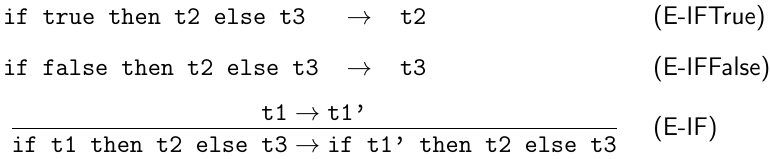
\includegraphics[width=9cm]{evaluation_bool_ch3}
\end{center}

\begin{center}
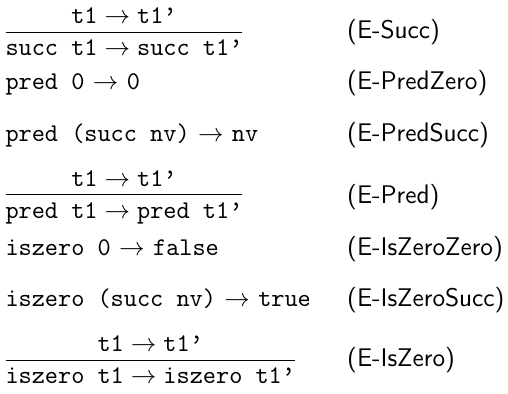
\includegraphics[width=6cm]{evaluation_numeric_ch3}
\end{center}

\end{frame}

%%%
\begin{frame}[t]{Summary: The arithmetic PL - Derivations}  \vspace{10pt}

A derivation tree of height 3 defines the semantics \\
\ \ \ for a single step ``\texttt{pred (succ (pred 0)) $\rightarrow$ pred (succ 0)}'' \\
\ \ \ using the three rules: (E-PredZero), (E-Succ), and (E-Pred).

\vspace{10pt}

\begin{center}
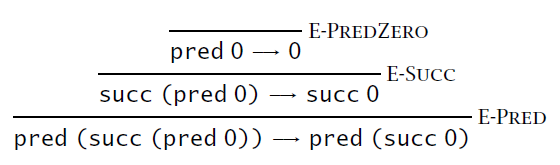
\includegraphics[width=8cm]{derivation_ch3}
\end{center}

\end{frame}

\begin{frame}[t]{Summary: The arithmetic PL - Semantics} \vspace{10pt}

The semantics of the airthmetic PL by constructing derivation trees

\vspace{10pt}

\begin{itemize}
\item One-step: A term \texttt{t1} evalutes to another \texttt{t2}\\
if you can derive \texttt{t1 $\rightarrow$ t2} by the ten evaluation rules.
\item Normal execution: A term \texttt{t1} normally evaluates to a value \\
if \texttt{t1 $\rightarrow^*$ v}
\item Runtime error: A term \texttt{t1} will get stuck at \texttt{t2} \\ if \texttt{t1 $\rightarrow^*$ t2}.
\end{itemize}

\vspace{10pt}

Thus the existence of a derivation tree constructed by the evaluation rules defines the semantics. 

\end{frame}

%%%
\begin{frame}[t]{Summary: The arithmetic PL - Induction} \vspace{10pt}

Q. Show that if \texttt{t $\rightarrow$ t1} and \texttt{t $\rightarrow$ t2} then \texttt{t1 = t2}.

\vspace{10pt}

By the induction, we can prove the uniqueness property for all infinite number of derivation trees for \texttt{t $\rightarrow$ t1}.

\vspace{10pt}

Proof by structural induction on the derivation of \texttt{t $\rightarrow$ t1}. 

\vspace{10pt}

\begin{itemize}
\item Base cases: The derivation trees of height 1.
\item Inductive cases: 
\begin{itemize}
\item[(1)] Assume the property to show is true for all the derivation trees of height $k$. 
\item[(2)] Then prove that the property is also true for all the derivation trees of height $k+1$.
\end{itemize}
\end{itemize}

\end{frame}


\end{document}
